\chapter{Введение}
Целью выполнения данной курсовой работы является ознакомление с процессом синтеза новых решений и 
освоение методов, используемых при проектировании новых технических решений.
Цель включает в себя несколько подцелей:
\begin{enumerate}
    \item Изучение конструктивно-функционального анализа технических объектов и получение навыков работы 
        с данным методом при проектировании новой техники.
    \item Изучение метода анализа технических решений, функционально -- физического анализа. 
    \item Получение навыков работы с автоматизированной системой поиска физических эффектов.
    \item Получение навыков работы с фондом эвристических приемов.
    \item Получение навыков работы с фондом эвристических приемов разрешения конфликтов.
    \item Получение навыков синтеза новых решений на основе фонда эвристических приемов, фонда 
        эвристических приемов разрешения конфликтов, анализа инверсных операций Коллера.
\end{enumerate}

\chapter{Концептуальное описание прототипа}
В последнее время пробки на дорогах становятся одной из важнейших проблем в современном мире. Число 
автомобилей с каждым годом растёт, а изменения в дорожной сети делаются в первую очередь для 
индивидуального транспорта, а не для общественного. Это ведёт к тому что с каждым днём будет становиться 
труднее попасть в ту или иную часть города, общественный транспорт -- устаревать, а машины -- парковаться 
в неположенных местах. Неудобные маршруты общественного транспорта -- зачастую сдерживающий фактор его 
использования. Нужно, чтобы прокладываемые маршруты в городе учитывали предпочтения обычный жителей, таких, 
как вы и я. 

Изменения в городской среде требуют формирования новых механизмов планирования инфраструктуры города. 
Для получения эффективных результатов, следует осуществлять принятие решений на основе актуальных данных, 
отражающих предпочтения жителей.

Главной особенностью данного прототипа является -- построение оптимальных маршрутов общественного 
транспорта, которые бы учитывали потребности жителей по перемещению в городе. 

Выделим основной функционал, которым должен обладать прототип:
\begin{itemize}
    \item генерации маршрута по предпочтениям жителей:
    \begin{itemize}
        \item алгоритм обхода кластеров предпочтений,
        \item алгоритм поиска пути между кластерами,
    \end{itemize}
    \item оценка эффективности построенных маршрутов:
    \begin{itemize}
        \item длина построенного маршрута,
        \item время в пути,
        \item кривизна маршрута.
    \end{itemize}
\end{itemize}

Модуль работает следующим образом. На вход подаются кластеризованные данные о предпочтении жителей в виде 
матрицы перемещений жителей от кластера к кластеру. Алгоритм обхода кластеров предпочтений формирует 
указанное количество маршрутов. Далее эти маршруты переходят на следующую стадию, где алгоритм поиска 
пути строит оптимальный маршрут между кластерами. На выходе мы получаем набор построенных маршрутных 
путей которые должны получить оценку -- насколько эффективными они являются. И наконец готовые маршруты 
строятся на карте.

\chapter{Конструктивно-функциональный анализ}
Конструктивно-функциональная структура прототипа представлена в таблице 1\\

Таблица 1. Конструктивно-функциональная структура прототипа
\begin{figure}[h!]
    \center
    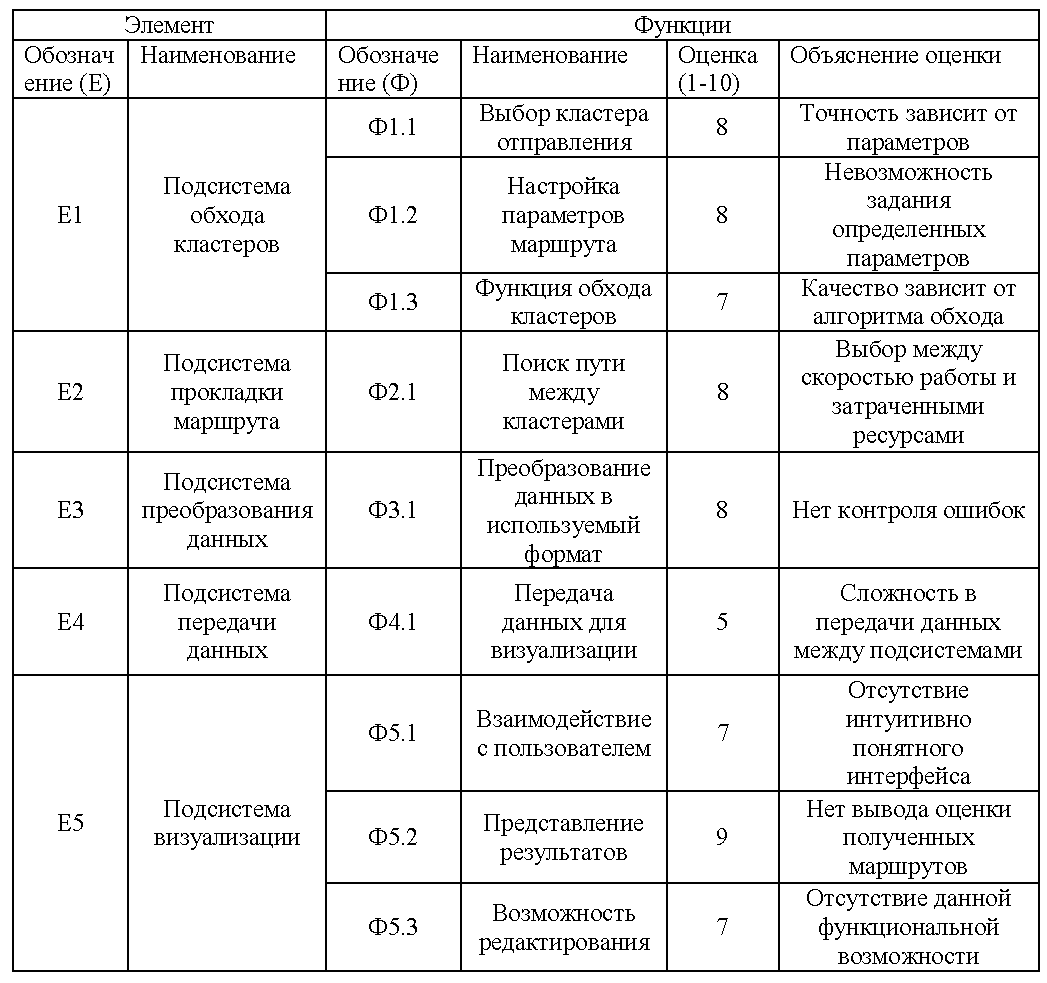
\includegraphics[width=\textwidth]{table01}
\end{figure}

\pagebreak

\noindent Недостатки:
\begin{itemize}
    \item Качество полученных маршрутов сильно зависит от используемого метода
    \item Нет возможности варьировать параметры генерации маршрутов
    \item Отсутствие интуитивно понятного интерфейса
    \item Отсутствие контроля ошибок
    \item Отсутствие возможности редактировать построенный маршрут
\end{itemize}
Цель работы:
\begin{itemize}
    \item Реализовать метод построения маршрутов с варьируемыми параметрами генерации
    \item Реализовать контроль данных
    \item Сделать интерфейс более наглядным
    \item Реализовать возможность редактирования маршрута
\end{itemize}

\chapter{Потоково-функциональный анализ}
Потоковая функциональная структура прототипа 
\begin{figure}[h!]
    \center
    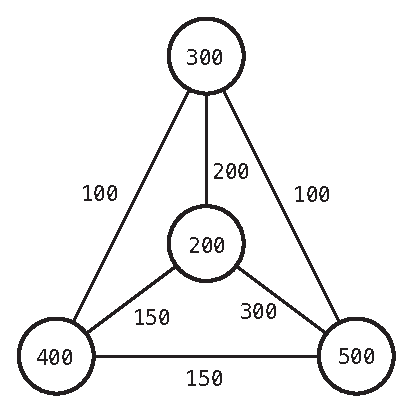
\includegraphics[width=0.6\textwidth]{img01}
\end{figure}

\begin{figure}[ht!]
    \center
    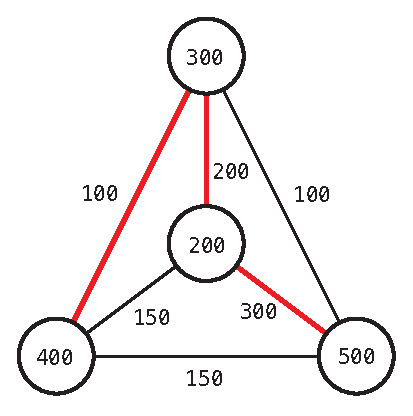
\includegraphics[width=0.8\textwidth]{img02}
    \caption{Конструктивно-функциональная структура прототипа в виде графа}
\end{figure}

\pagebreak

Таблица 2. Потоковая функциональная структура прототипа
\begin{figure}[h!]
    \center
    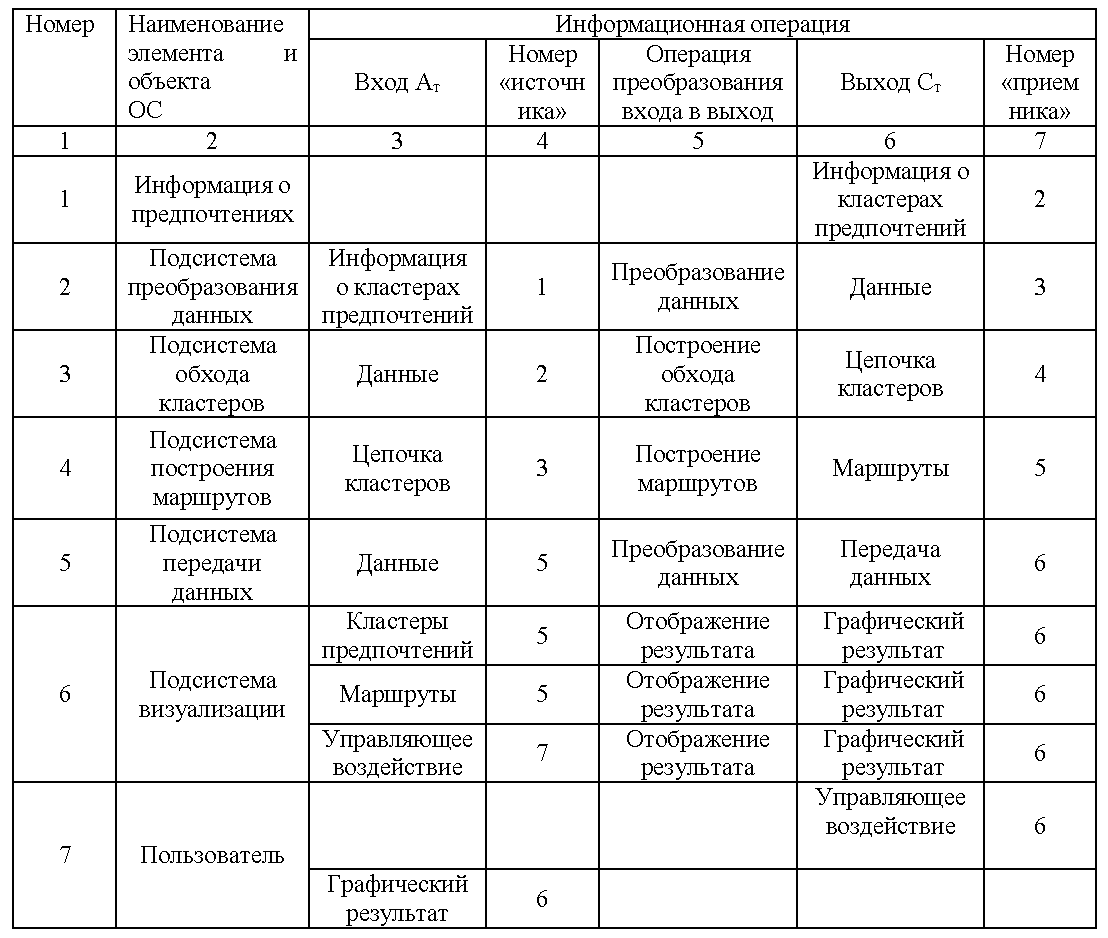
\includegraphics[width=\textwidth]{table02}
\end{figure}

\chapter{Функционально-физический анализ прототипа, оценка целостности}
\emph{Конструктивно-функциональный анализ, операции Коллера.}

Операции Коллера представлены в таблице 3.

Таблица 3. Операции Коллера
\begin{figure}[h!]
    \center
    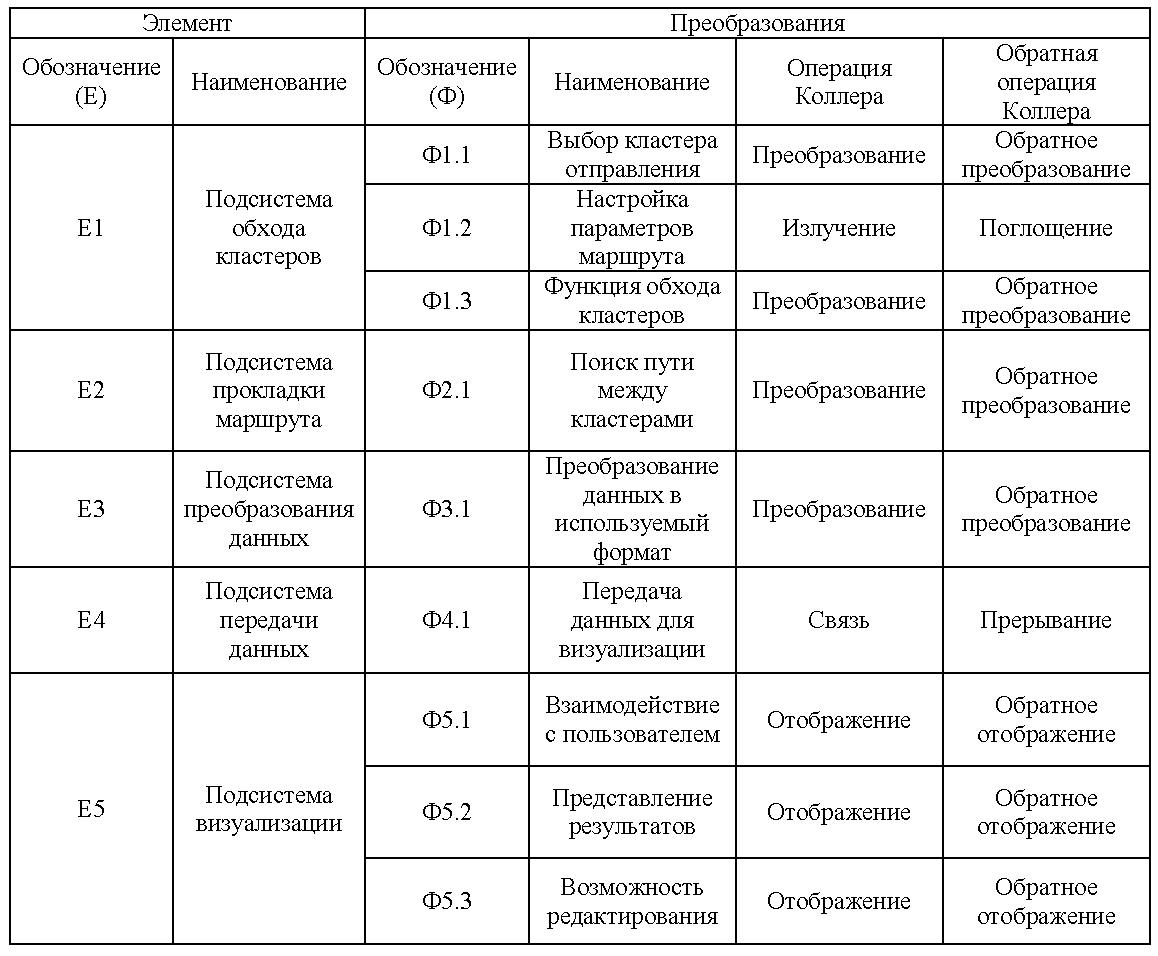
\includegraphics[width=\textwidth]{table03}
\end{figure}

\pagebreak

Таблица 4. Описание прототипа как информационной системы
\begin{figure}[h!]
    \center
    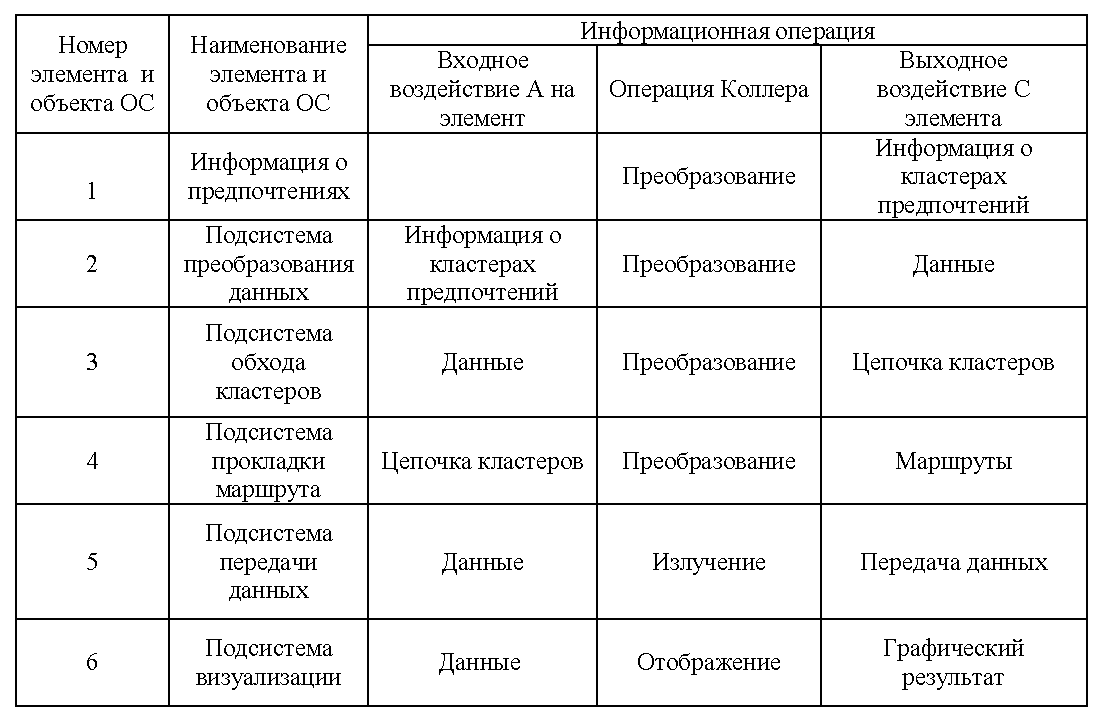
\includegraphics[width=\textwidth]{table04}
\end{figure}

\emph{Диаграмма Исикавы}
\begin{figure}[h!]
    \center
    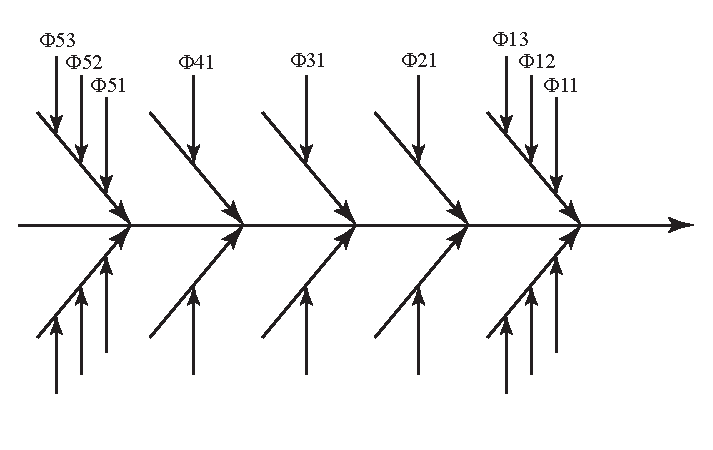
\includegraphics[width=0.7\textwidth]{img03}
    \caption{Диаграммы Исикавы для главной функции и для операций Колера (инвертированные функции снизу).}
\end{figure}

\chapter{Синтез новых технических решений на основе использования эвристических приемов, 
    оценка новизны решений}
Синтез новых решений с использованием ЭП приведен в таблице 5 и 6.

Таблица 5. Синтез новых решений с использованием ЭП
\begin{figure}[h!]
    \center
    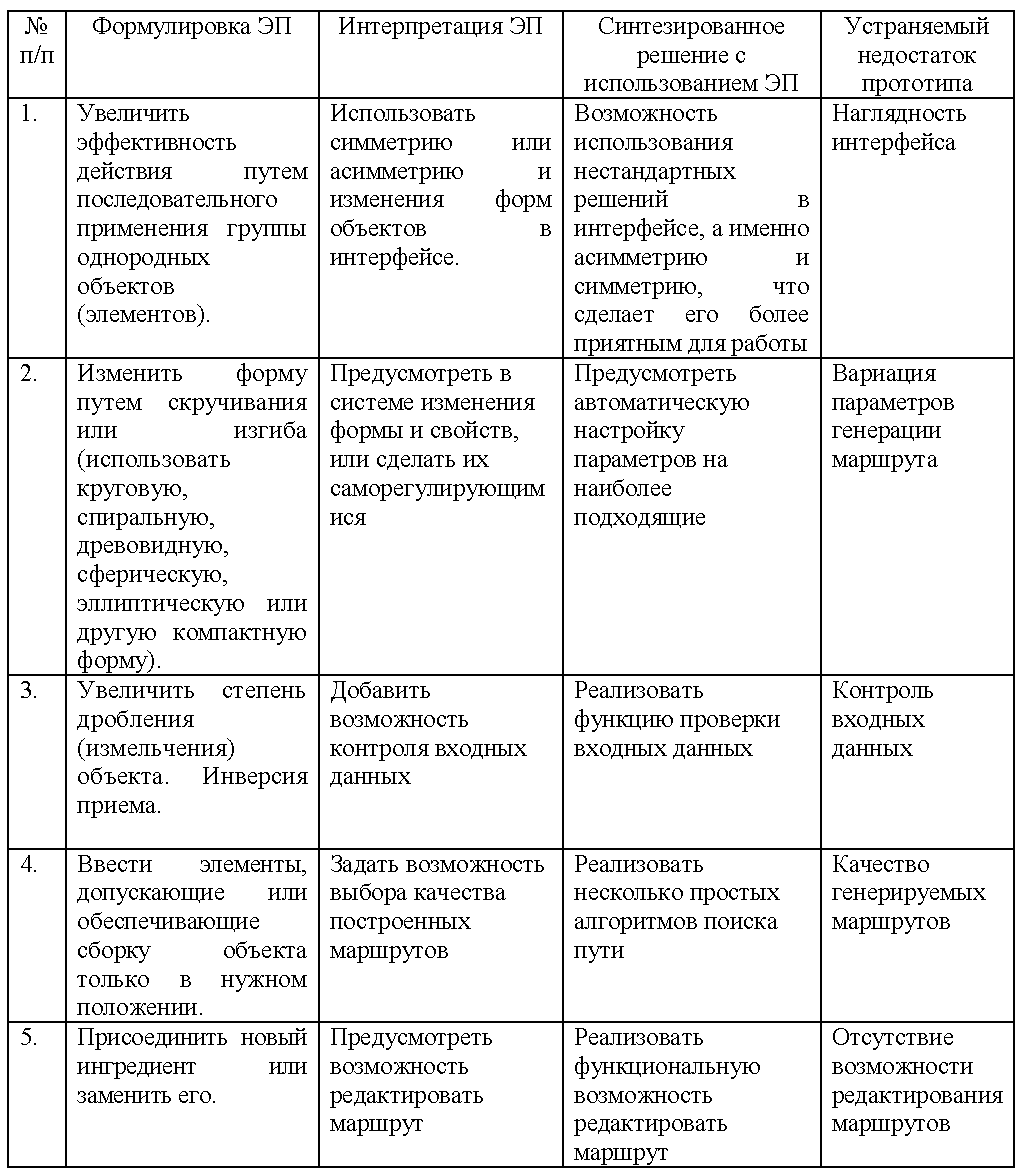
\includegraphics[width=\textwidth]{table05}
\end{figure}

\pagebreak

Таблица 6. Синтез новых решений с использованием инвертированных ЭП
\begin{figure}[h!]
    \center
    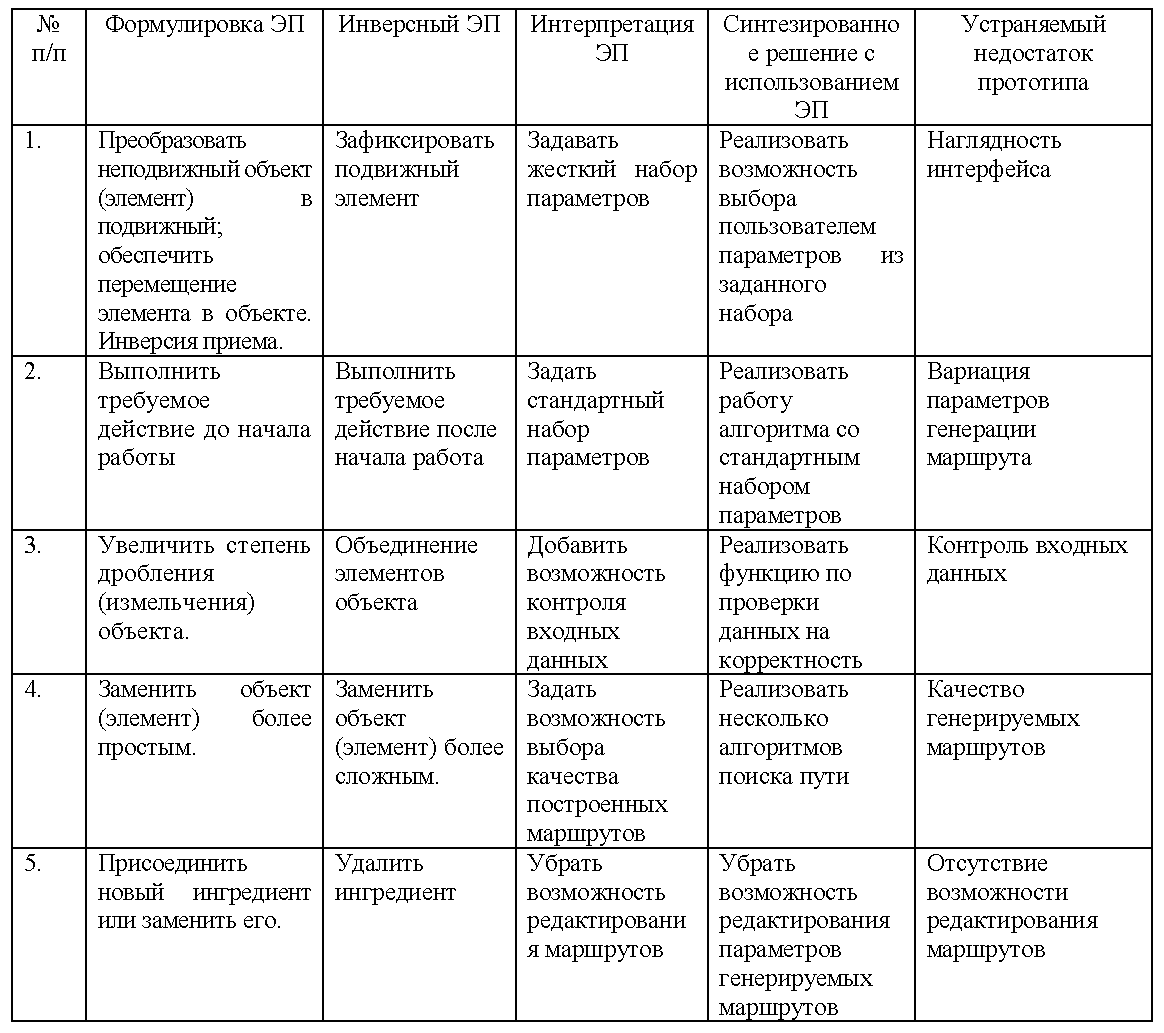
\includegraphics[width=\textwidth]{table06}
\end{figure}

\pagebreak

Таблица 7. Сравнение прототипа и синтезированных решений. 
\begin{figure}[h!]
    \center
    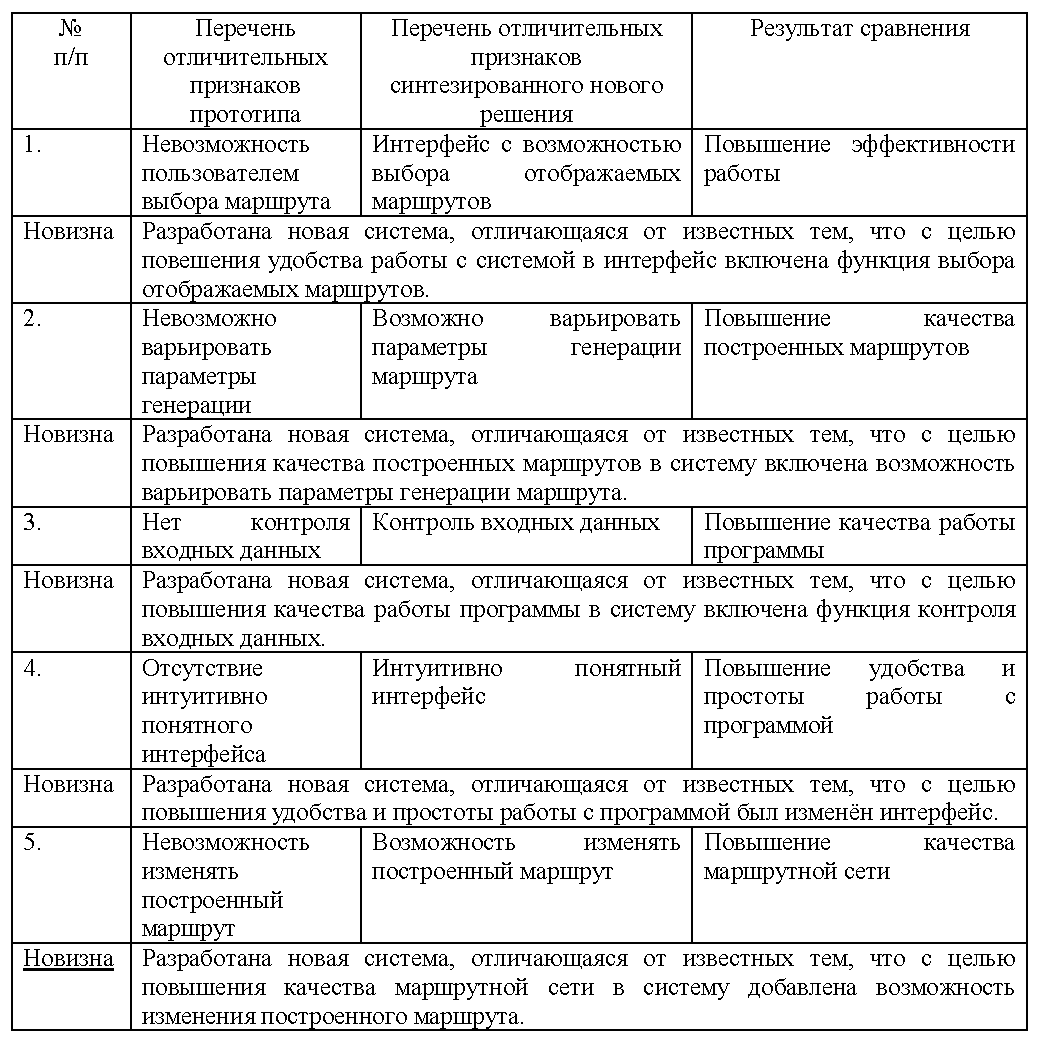
\includegraphics[width=\textwidth]{table07}
\end{figure}

\chapter{Постановка задачи поиска нового технического решения с описанием синтезированных решений и 
    оценкой их новизны}
Решение 1.
\begin{enumerate}
    \item Недостаточная наглядность интерфейса
    \item Подсистема визуализации
    \item Экранная форма
    \item Изменение параметра
    \begin{itemize}
        \item Отрисовка выбранного маршрута;
        \item Внесение изменений в маршрут.
    \end{itemize}
    \item Конфликт между показателями качества: П1 -- наглядность работы системы, 
        П2 -- загруженность интерфейса. Повышение наглядности работы системы приводит к 
        перегруженности интерфейса.
    \item Функциональный конфликт: Ф1 -- функция наглядности работы системы, Ф2 -- 
        функция загруженности.
    \item Конфликт свойств. С1 -- интерфейс должен поддерживать возможность выбора отображаемого 
        маршрута. С2 -- интерфейс не должен поддерживать возможность выбора отображаемого маршрута.
    \item Изменение системы. Заменить узловой элемент объектом, который на различных стадиях (фазах) 
        жизненного цикла исходной системы он характеризовался различными значениями параметра, 
        указанного в формуле конфликта свойств.
    \item Решение. Отображение наилучшего маршрута по оценочным критериям.
\end{enumerate}

\pagebreak

Решение 2.
\begin{enumerate}
    \item Недостаток -- отсутствие возможности редактирования маршрута
    \item Подсистема визуализации
    \item Экранная форма
    \item Изменение параметра
    \begin{itemize}
        \item Выбор редактируемого маршрута;
        \item Изменение контрольных точек.
    \end{itemize}
    \item Конфликт между показателями качества: П1 -- качество маршрута, 
        П2 -- сложность реализации. Повышение качества маршрутной сети системы приводит к сложности 
        реализации функционала.
    \item Функциональный конфликт: Ф1 -- функция качества, Ф2 -- 
        функция сложности.
    \item Конфликт свойств. С1 -- интерфейс должен поддерживать возможность редактирования маршрута. 
        С2 -- интерфейс не должен поддерживать возможность редактирования маршрута.
    \item Изменение системы. Заменить узловой элемент объектом, который на различных стадиях (фазах) 
        жизненного цикла исходной системы он характеризовался различными значениями параметра, 
        указанного в формуле конфликта свойств.
    \item Решение. Реализовать построение нескольких вариаций маршрутов.
\end{enumerate}

\pagebreak

Синтезировать новые решения с помощью процедур постановки задачи поиска нового технического решения 
для реализации инверсных операций Коллера по результатам конструктивно-функционального анализа:

Решение 3.\\
\emph{Элемент} -- подсистема обхода кластеров.\\
\emph{Операция Коллера} -- преобразование.\\
\emph{Инверсная операция Коллера} -- обратное преобразование.\\
Реализовать возможность вариации основных параметров системы.\\

Решение 4.
\emph{Элемент} -- подсистема преобразования данных.\\
\emph{Операция Коллера} -- преобразование.\\
\emph{Инверсная операция Коллера} -- обратное преобразование.\\
Реализовать возможность контроля данных на ошибки.\\

Решение 5.
\emph{Элемент} -- подсистема преобразования данных.\\
\emph{Операция Коллера} -- преобразование.\\
\emph{Инверсная операция Коллера} -- обратное преобразование.\\
Реализовать возможность контроля данных на ошибки.\\

Оценить новизну полученных решений на основе сравнения отличительных признаков прототипа и нового решения. 
В результате работы синтезировано 5 новых решений.

\chapter{Синтез заставки}
1. Гирлянда синонимов к слову путь: дорога, ход, движение, курс.

2. Случайные объекты: ковёр, бумага, монета, ручка.

3. Составление комбинаций из элементов гирлянды синонимов объекта и элементов гирлянды случайных объектов:

Дорожный ковёр, дорожная бумага, дорожная монета, дорожная ручка, ходящих ковёр, ходовая бумага, 
ходовая монета, ходовая ручка, движение ковёр, движущаяся бумага, движение монет, двигающаяся ручка, 
курсирующий ковёр, курс бумаги, курс монеты, курс ручки.

4. Составление признаков случайных объектов:
\begin{table}[h!]
    \center
    \begin{tabularx}{\textwidth}{|X|X|}
        \hline
        Объект & Признаки \\ \hline
        ковёр & мягкий, пушистый, красивый \\ \hline
        бумага & мятая, старая, дорогая \\ \hline
        монета & винтажная, древняя, обычная \\ \hline
        ручка & удобная, шариковая, дверная \\ \hline
    \end{tabularx}
\end{table}

5. Генерирование идей путем поочередного присоединения к техническому объекту и его синонимам 
признаков случайно выбранных объектов:
\begin{table}[h!]
    \center
    \begin{tabularx}{\textwidth}{|X|X|}
        \hline
        Дорога & мягкая дорога, пушистая дорога, красивая дорога, мятая дорога, старая дорога, 
            дорогая дорога, винтажная дорога, древняя дорога, обычная дорога, удобная дорога, 
            шариковая дорога, дверная дорога \\ \hline
        Ход & мягкий ход, пушистый ход, красивый ход, мятый ход, старый ход, дорогой ход, 
            винтажный ход, древний ход, обычный ход, удобный ход, шариковый ход, 
            дверной ход \\ \hline
        Движение & мягкое движение, пушистое движение, красивое движение, мятое движение, 
            старое движение, дорогое движение, винтажное движение, древнее движение, 
            обычное движение, удобное движение, шариковое движение, дверное движение \\ \hline
        Курс & мягкий курс, пушистый курс, красивый курс, мятый курс, старый курс, дорогой курс, 
            винтажный курс, древний курс, обычный курс, удобный курс, шариковый курс, 
            дверной курс \\ \hline
    \end{tabularx}
\end{table}

6. Генерирование гирлянд ассоциаций

\begin{table}[h!]
    \center
    \begin{tabularx}{\textwidth}{|X|X|}
        \hline
        мягкий & диван, кровать, подушка \\ \hline
        пушистый & кот, палас, зверь \\ \hline 
        красивый & автомобиль, код, клавиатура \\ \hline
        мятая & салфетка, кресло, подушка \\ \hline
        старая & книга, переплёт, часы \\ \hline
        дорогая & покупка, техника, игра \\ \hline
        винтажный & пистолет, компьютер, стол \\ \hline
        древний & руины, пирамида, река \\ \hline
        обычный & человек, время, дело \\ \hline
        удобный & носки, посуда, кровать \\ \hline
        шариковый & механизм, мышь, трекболл \\ \hline
        дверной & замок, глазок, проём \\ \hline
    \end{tabularx}
\end{table}

7. Генерирование новых идей: мягкий пушистый диван, пушистый красивый кот, пушистый винтажный кот, 
красивый мятый автомобиль, красивая старая клавиатура, красивый винтажный код, мятое старое кресло, 
мятая дорогая подушка, старая дорогая книга, старый винтажный переплёт, старая обычная книга, 
дорогая винтажная покупка, дорогая древняя игра, винтажный древний пистолет, шариковый дверной механизм.

8. Выбор рациональных вариантов: мягкий пушистый диван, старый винтажный переплёт, 
винтажный древний пистолет, шариковый дверной механизм.

9. Окончательный синтез заставки. Кот запрыгнул на мягкий пушистый диван. Человек подбирает книги со 
старым винтажным переплётом для своей коллекции. Шариковый дверной механизм -- самый надёжный механизм.

\chapter{Выводы}
В ходе выполнения работы были реализованы различные методы создания технических решений для 
поиска пути на графе дорог. Реализованы следующие этапы синтеза новых технических решений: 
\begin{enumerate}
    \item Конструктивно-функциональный анализ прототипа. На этом этапе система декомпозируется на 
        элементы, описываются функции элемента и приводится оценка этих функций 
        (конструктивно-функциональная структура прототипа). Это необходимо для определения недостатков 
        прототипа и постановки целей совершенствования системы. Далее приводится потоковая структура 
        прототипа для описания информационных процессов, происходящих в системе. Приводится 
        конструктивно-функциональная структура в виде графа, на которой отображаются элементы 
        системы и их функции. 
    \item Функционально-информационный анализ прототипа. Этот этап необходим для определения 
        операций Коллера, описания прототипа как информационной системы. 
    \item Построение диаграмм Исикавы по функционалу прототипа, определение целостности системы. 
        Этот этап необходим для выявления взаимосвязей между различными функциями системы, понимания 
        существенных факторов, которые влияют на работу системы, более глубокого понимания недостатков 
        системы. 
    \item Синтез новых решений по совершенствованию прототипа. Проведен синтез решений с использованием 
        эвристических приемов и инвертированных эвристических приемов. В результате этого этапа было 
        синтезировано 5 новых решений, которые позволяют повысить эффективность системы. 
    \item Постановка задачи поиска нового решения. На этом этапе поставлена задача поиска нового 
        решения с описанием новых синтезированных решений и оценкой новизны. Предложены решения по 
        реализации инверсных операций Коллера. 
    \item Разработана заставка, которая отображается при установке системы. 
        Содержание заставки следующее: Кот запрыгнул на мягкий пушистый диван. Человек подбирает 
        книги со старым винтажным переплётом для своей коллекции. Шариковый дверной механизм -- 
        самый надёжный механизм.
\end{enumerate}